\documentclass[aspectratio=1610]{beamer}

\usepackage[utf8]{inputenc}
\usepackage{graphicx}
\usepackage{amssymb}
\usepackage[export]{adjustbox}
\usetheme{Frankfurt}
\usefonttheme[onlymath]{serif}
\usepackage[super]{nth}
\graphicspath{{./Figure/}}
\usepackage{hyperref}
\usepackage{listings}
\hypersetup{
    colorlinks=true,
    linkcolor=blue,
    filecolor=magenta,      
    urlcolor=cyan,
}
\definecolor{satinsheengold}{rgb}{0.85, 0.63, 0.21}
\setbeamercolor{structure}{fg=satinsheengold}
\setbeamercolor{title}{fg=black}
\setbeamercolor{title in head/foot}{fg=black, bg=satinsheengold}
\setbeamercolor{author}{fg=black}
\setbeamercolor{frametitle}{fg=black}
\setbeamercolor{author in head/foot}{fg=black, bg=satinsheengold}
\setbeamercolor{institute in head/foot}{bg=satinsheengold}
\setbeamercolor{date in head/foot}{bg=satinsheengold}
\setbeamercolor{navigation symbols}{fg=gray}
\setbeamercolor{block title}{bg=black}
\setbeamercolor{item projected}{fg=black}
\setbeamertemplate{blocks}[rounded][shadow=false]
\setbeamertemplate{enumerate items}[circle]
%\setbeamertemplate{footline}[frame number]
%Adding frame #s
\setbeamertemplate{navigation symbols}{%
    \usebeamerfont{footline}%
    \usebeamercolor[fg]{footline}%
    \hspace{1em}%
    \insertframenumber/\inserttotalframenumber
}

\title{Coding Assignment 1 Write-up}
\author{Andrew Sivaprakasam}

\date{03/20/2021}


\begin{document}
\frame{\titlepage}

\begin{frame}
\frametitle{Question 2$|$ One-Way Sensitivity Analysis Tornado Plots}
\small{Observations of how sensitive the model output is to the specified parameters. }
\begin{center}
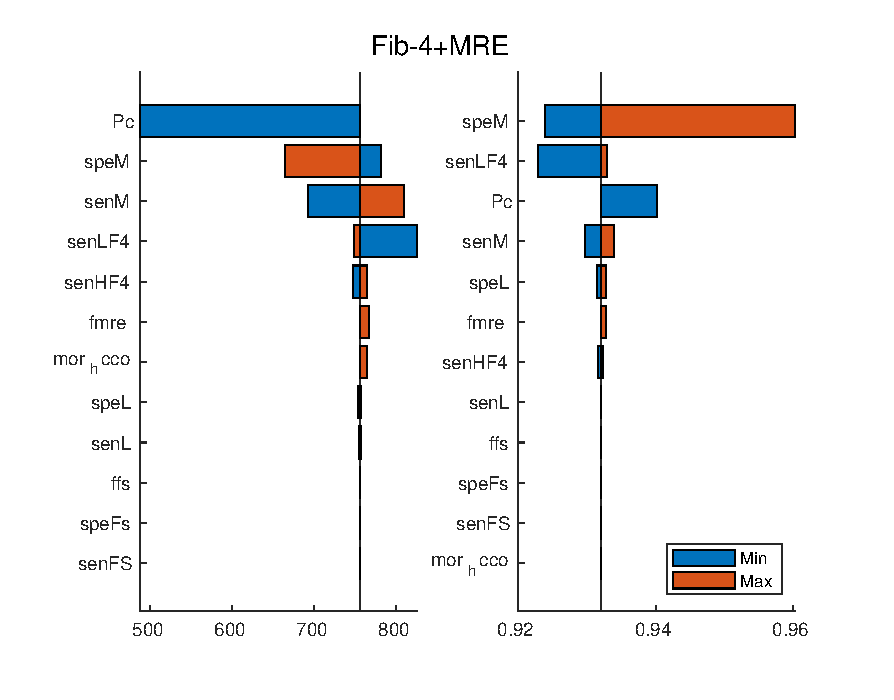
\includegraphics[width = .36\textwidth]{sens1}
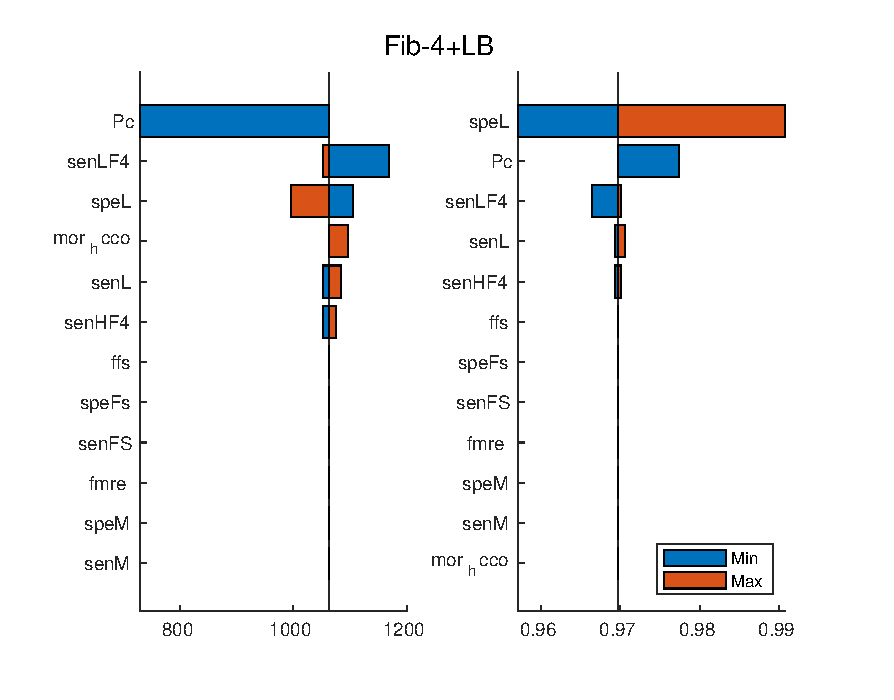
\includegraphics[width = .36\textwidth]{sens2}
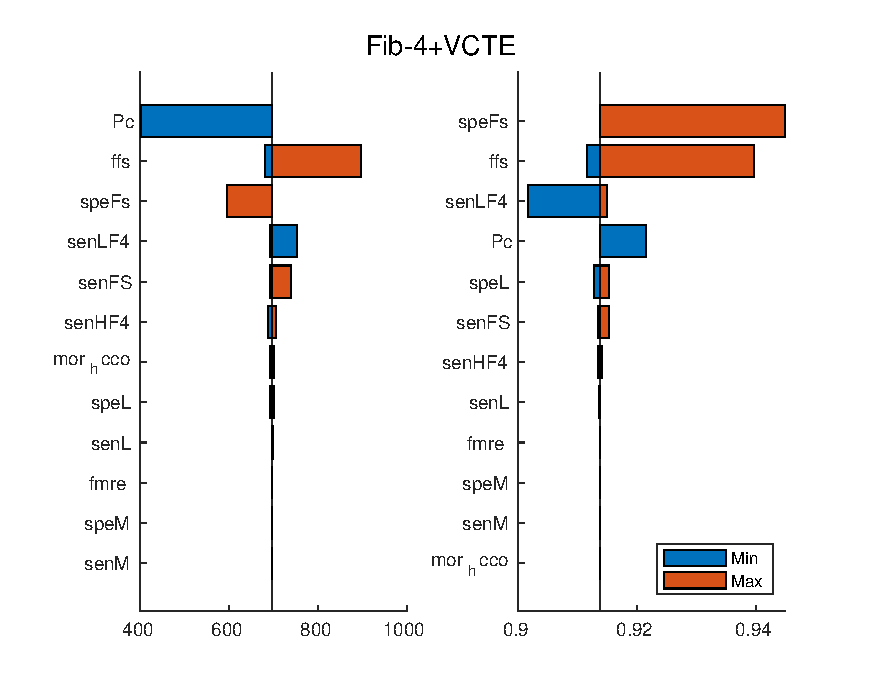
\includegraphics[width = .36\textwidth]{sens3}
\end{center}
\end{frame}

\begin{frame}
\frametitle{Question 3a$|$ Full-Factorial Histograms}

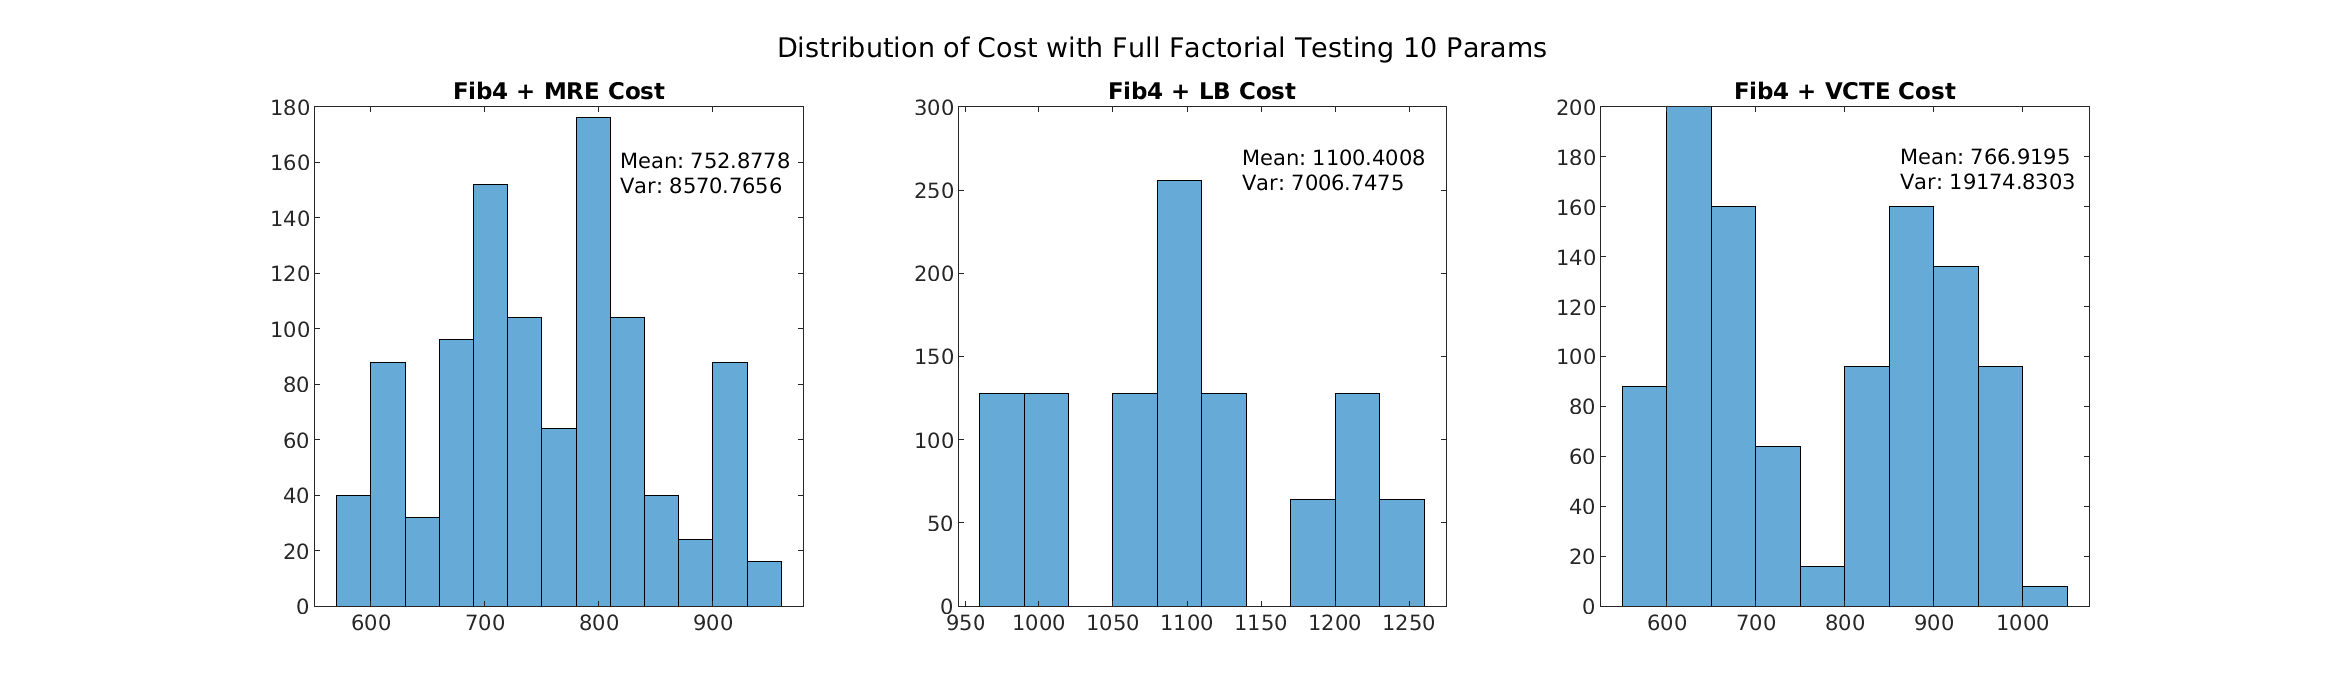
\includegraphics[width = \textwidth]{cost_distributions}
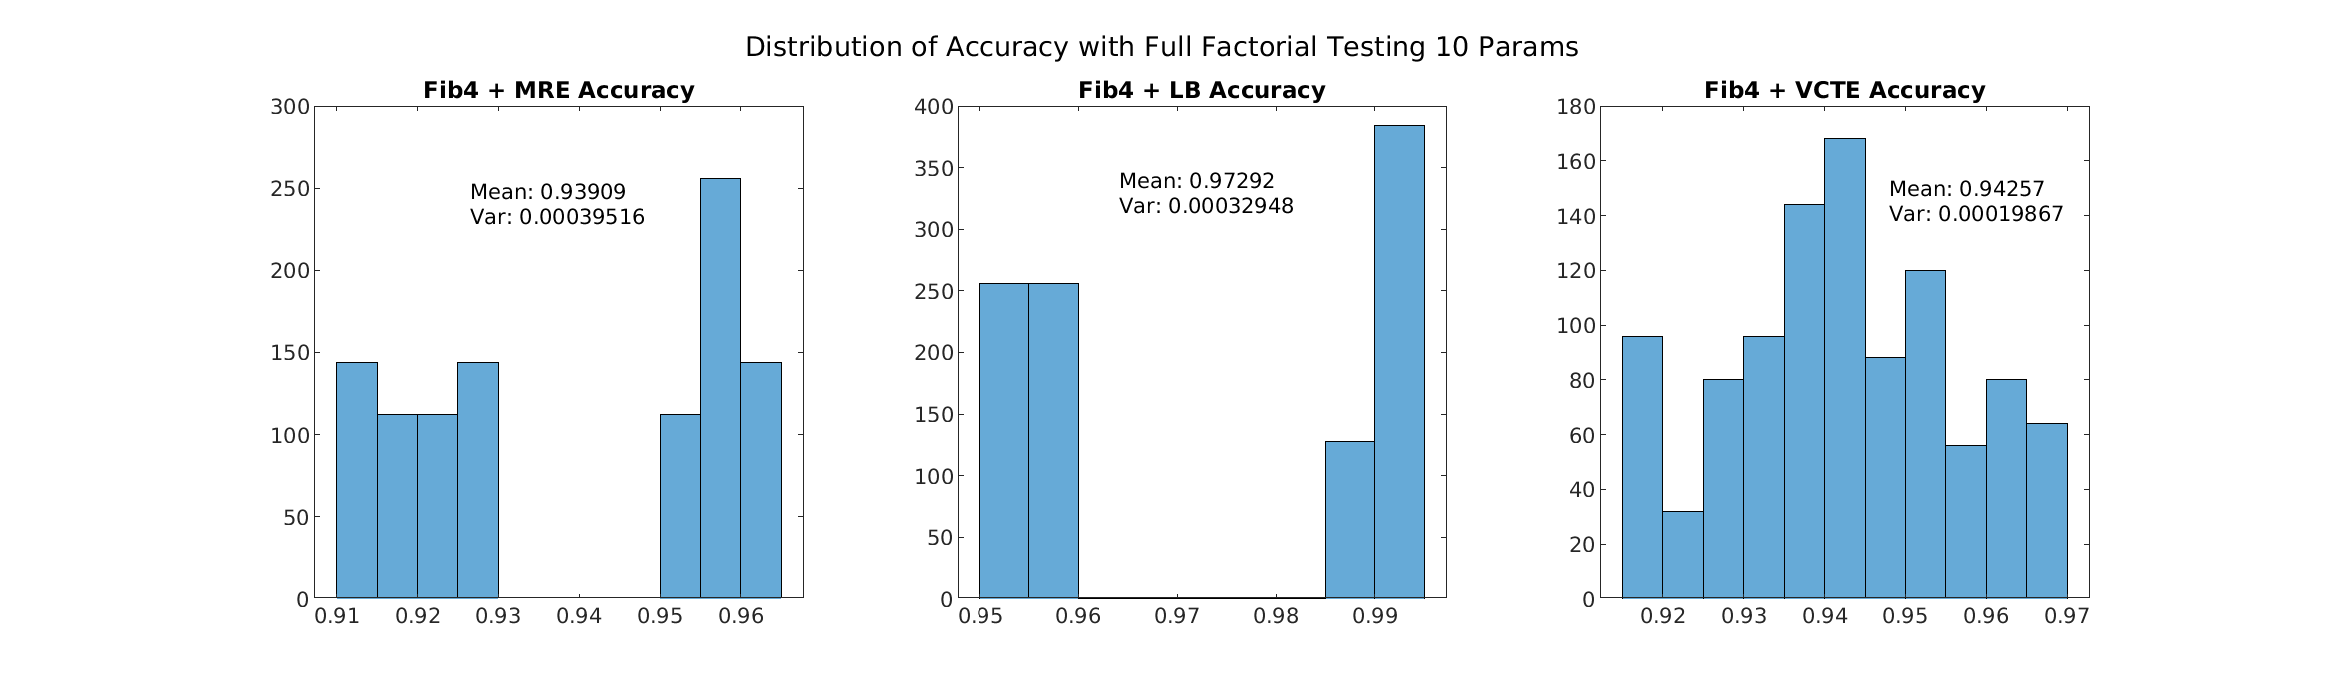
\includegraphics[width = \textwidth]{accuracy_distributions}

\end{frame}

\begin{frame}
\frametitle{Question 3a$|$ Full-Factorial Fitted Distributions}
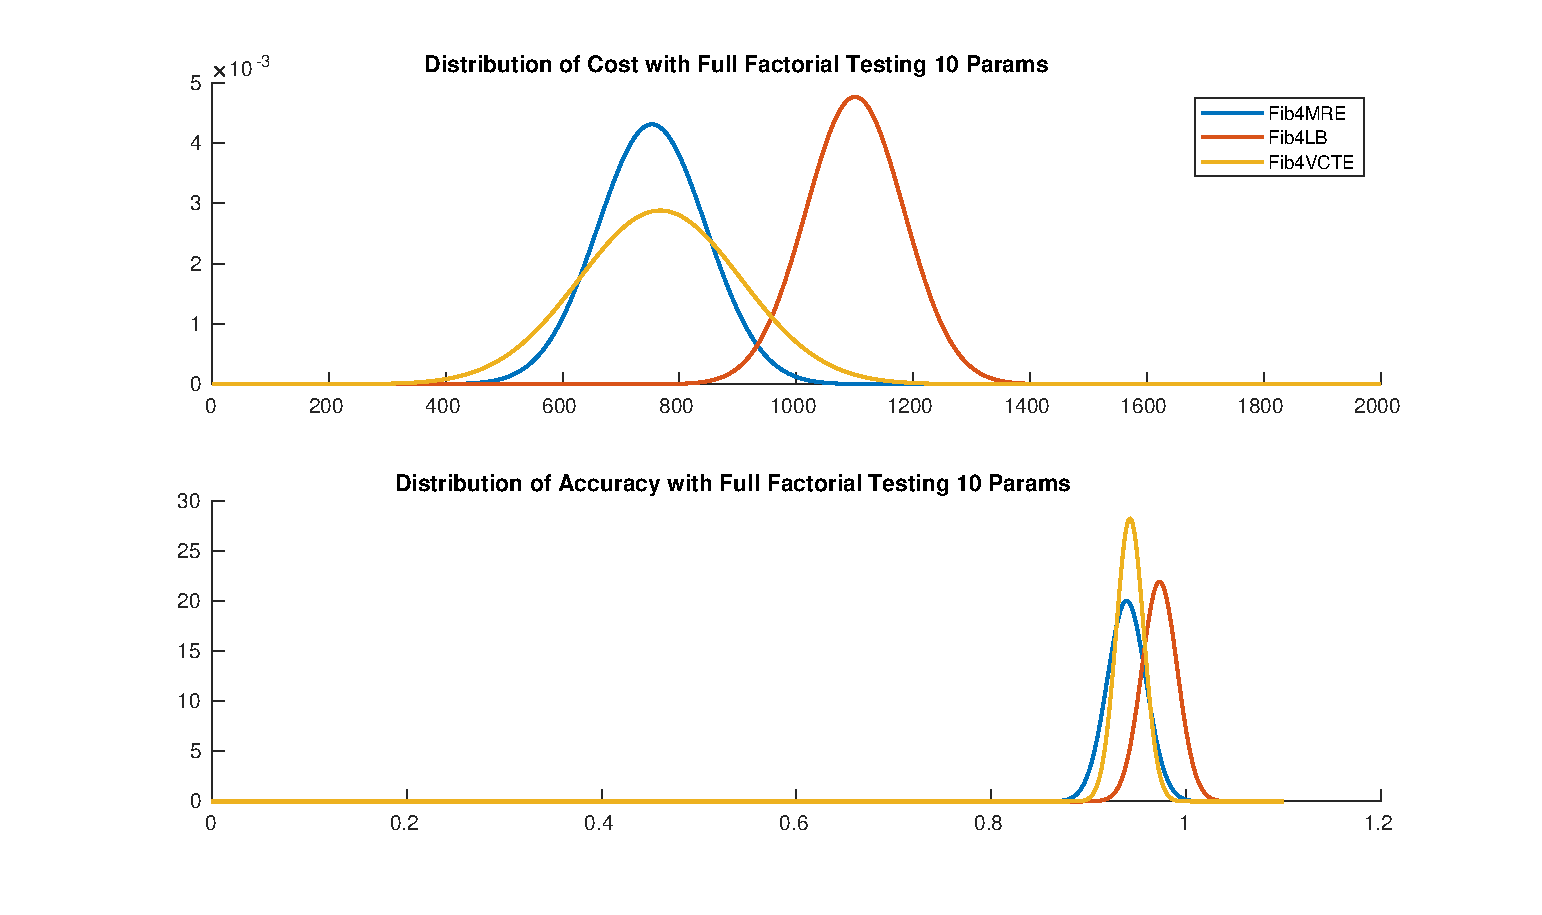
\includegraphics[width = \textwidth]{fitted_dist}
\end{frame}

\begin{frame}[fragile]
\frametitle{Question 3b$|$ Full-Factorial Percent > 300 (from Code)}
The percent of trials where the difference $|LB_{cost} - MRE_{cost}| > 300$ was \underline{61.7188}\%

\vspace{2em}
See \verb|q3.m|  252-253:

\begin{center}
\begin{verbatim}
diff = abs(Fib4MRE_cost_out-Fib4LB_cost_out);
percent_greater = sum(diff>300)*100/L;
\end{verbatim}
\end{center}
\end{frame}

\begin{frame}[fragile]
\frametitle{Question 3c$|$ Full-Factorial Sensitivity Analysis on \underline{MRE}}

The effect of varying MRE specificity and sensitivity params ( \verb|speM| \& \verb|senM| ) on the cost difference between MRE and LB can be visualized as follows:
\vspace{1.5em}

\centering
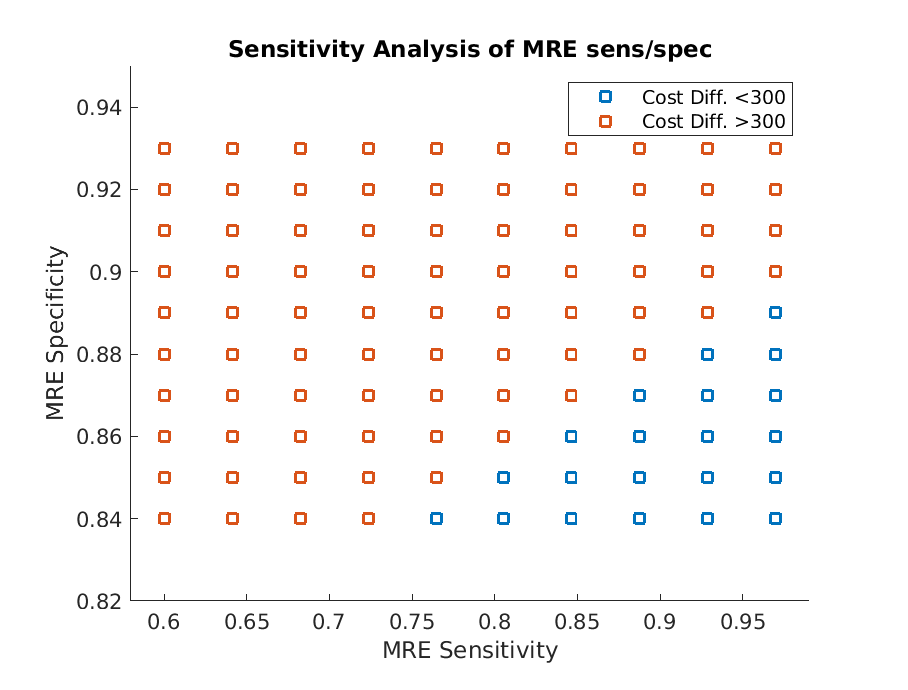
\includegraphics[width = .49\textwidth]{3c_1}
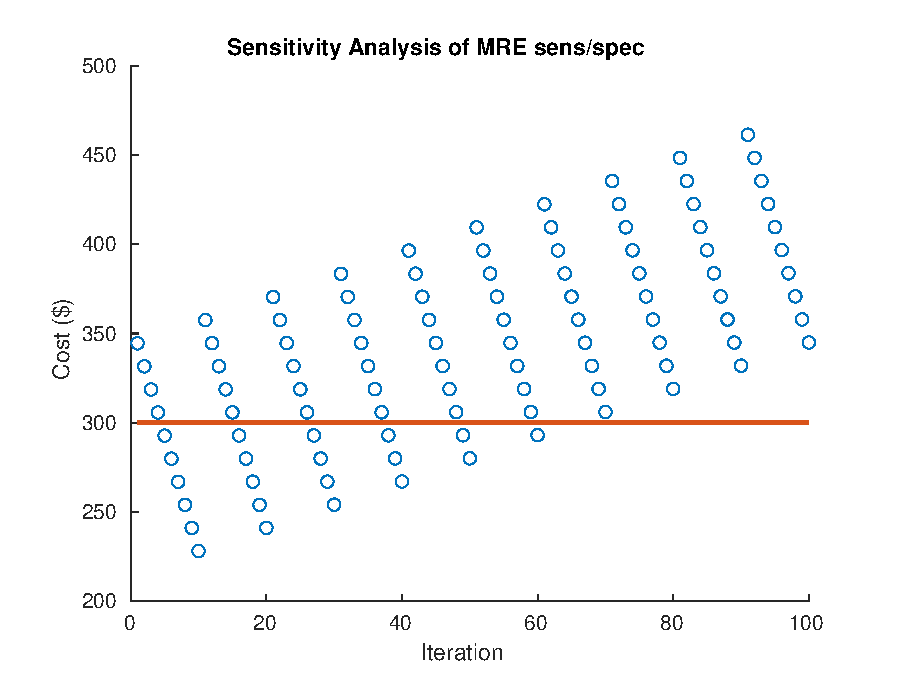
\includegraphics[width = .49\textwidth]{3c_2}

\textit{\underline{79\%} of the simulated outputs for cost difference were greater than 300.}

\end{frame}

\begin{frame}[fragile]
\frametitle{Question 3d$|$ Full-Factorial Sensitivity Analysis on \underline{LB}}

The effect of varying LB specificity and sensitivity params ( \verb|speM| \& \verb|senM| ) on the cost difference between MRE and LB can be visualized as follows:
\vspace{1.5em}

\centering
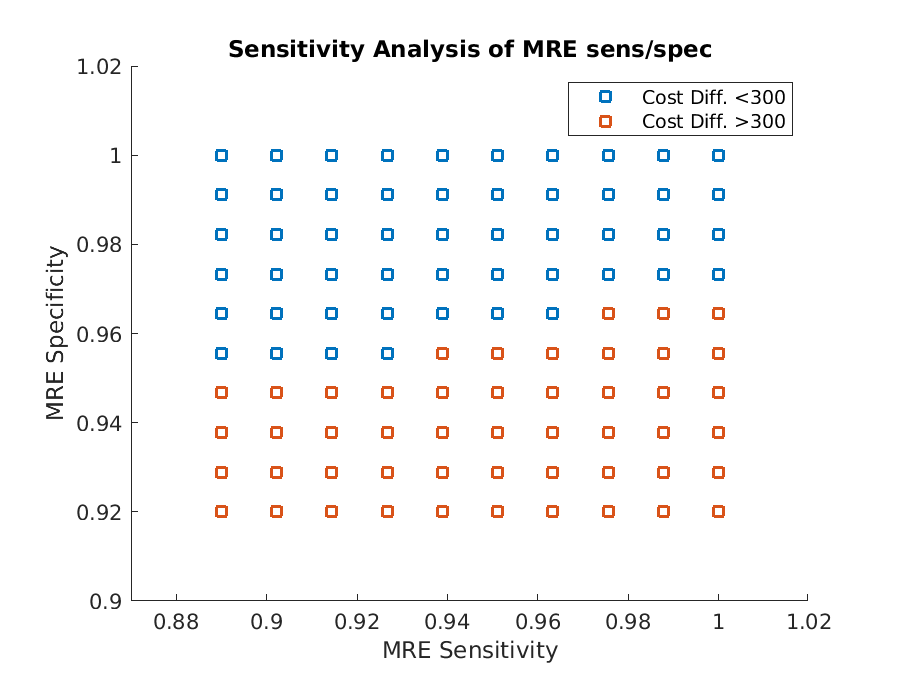
\includegraphics[width = .49\textwidth]{3d_1}
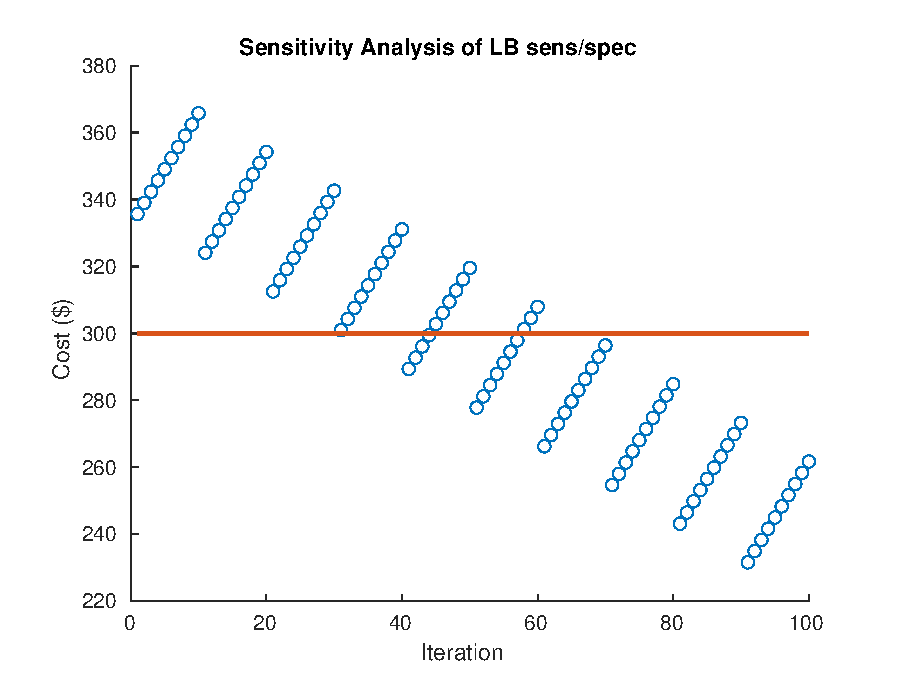
\includegraphics[width = .49\textwidth]{3d_2}

\textit{\underline{49\%} of the simulated outputs for cost difference were greater than 300.}

\end{frame}

\begin{frame}[fragile]
\frametitle{Sample-Based Sensitivity Analysis}
Here is a verification that my sampling was done correctly. I created a brute-force method for orthogonal sampling, \verb|orth_samples.m|. 

\vspace{1em}
\centering
\hspace*{-2cm}                                                           
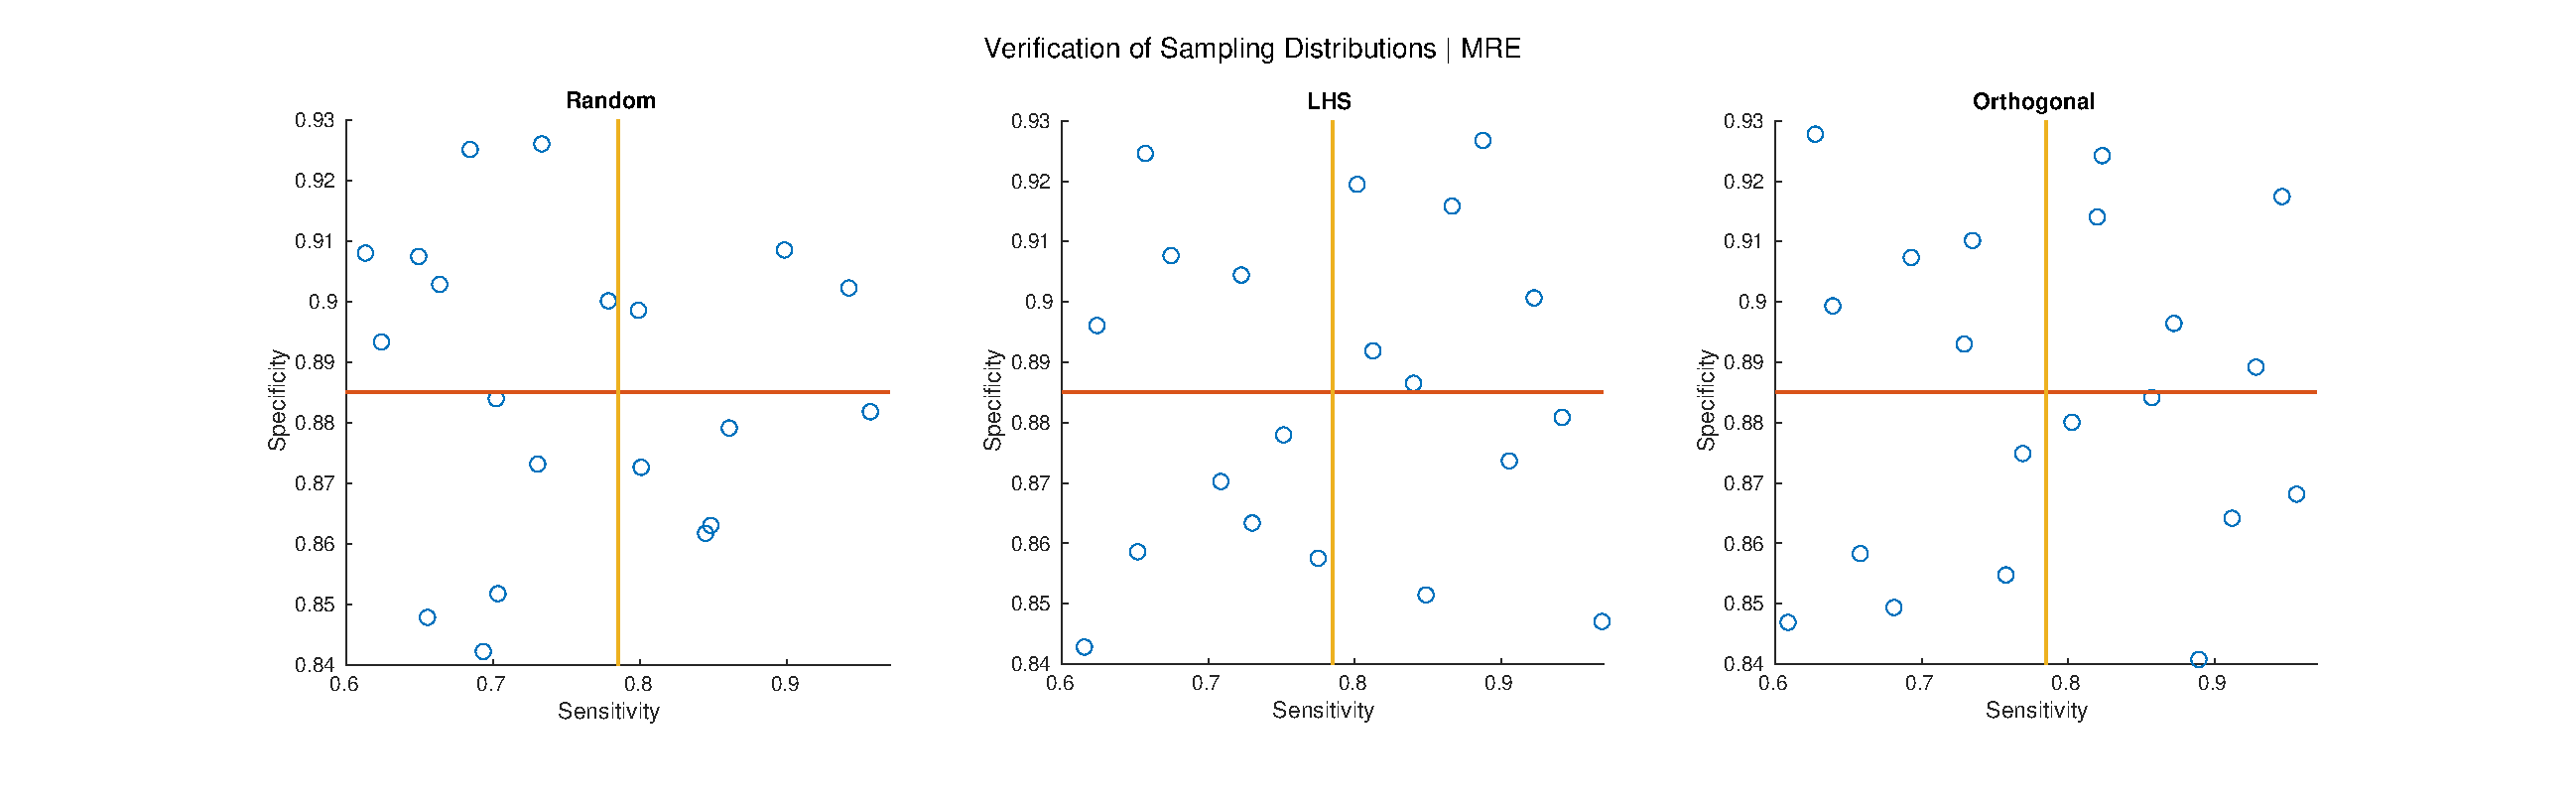
\includegraphics[scale = .41]{sampling_ex}
\end{frame}

\begin{frame}
\frametitle{Question 3e $|$ Sample-Based Sensitivity Analysis for \underline{MRE}}
Here are the 3D plots, regression equations and Pearson's correlation coefficients for the MRE sample-based Sensitivity Analysis. 

\vspace{1em}
\centering                                                         
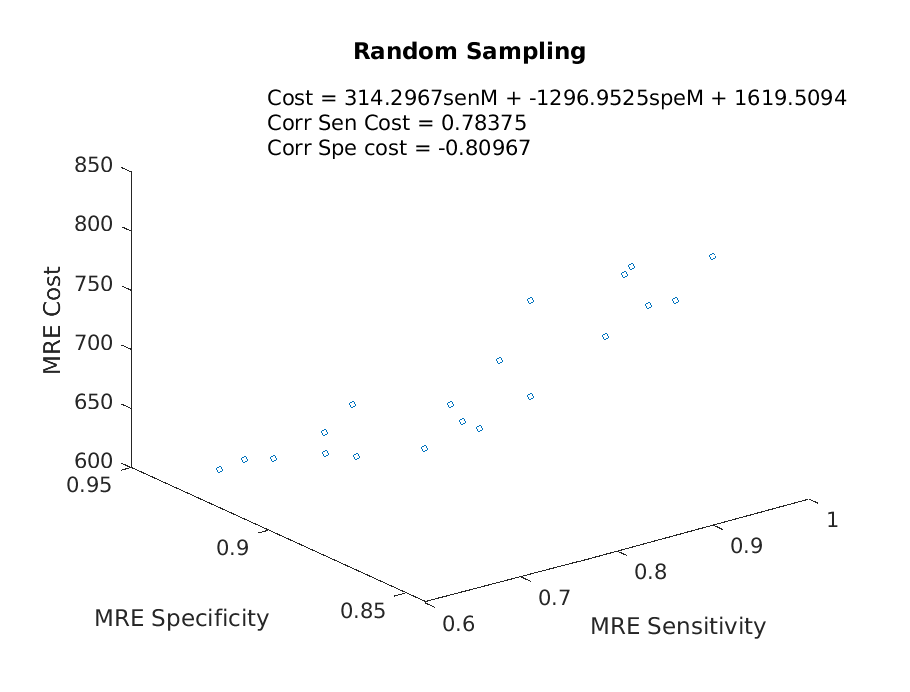
\includegraphics[scale = .3]{mre1}
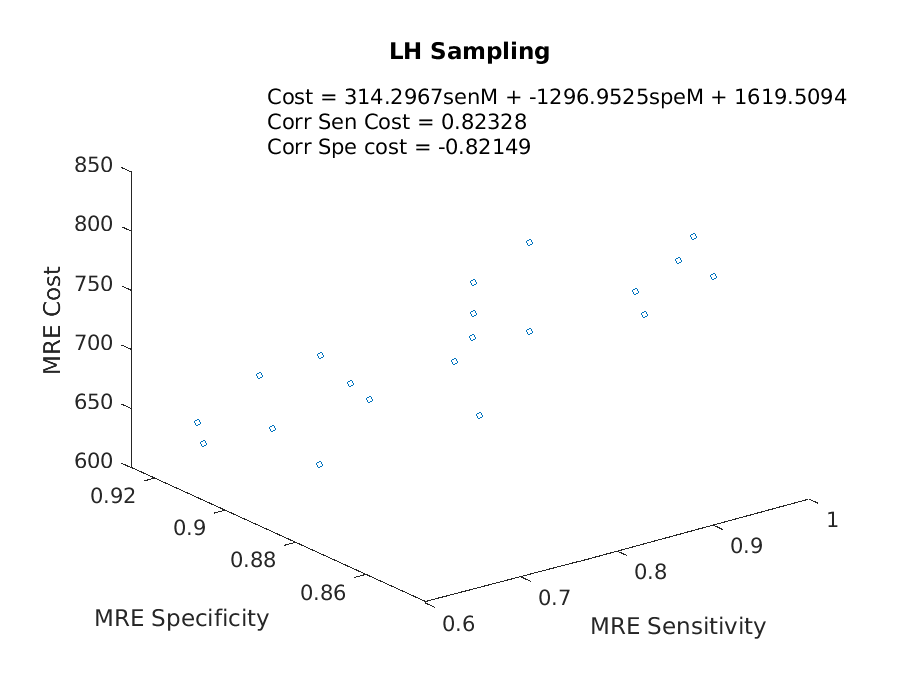
\includegraphics[scale = .3]{mre2}
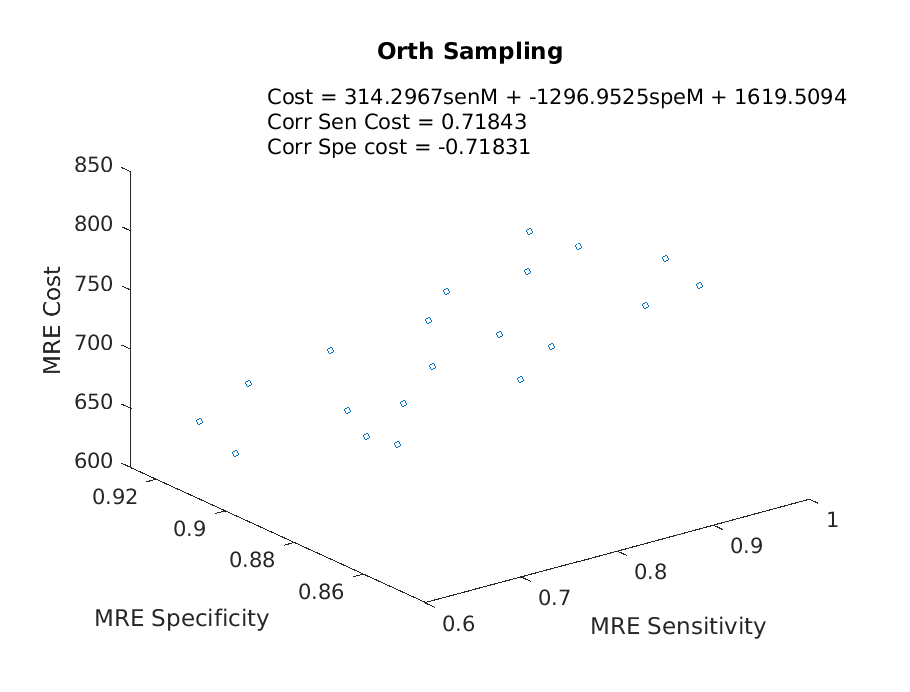
\includegraphics[scale = .3]{mre3}\\
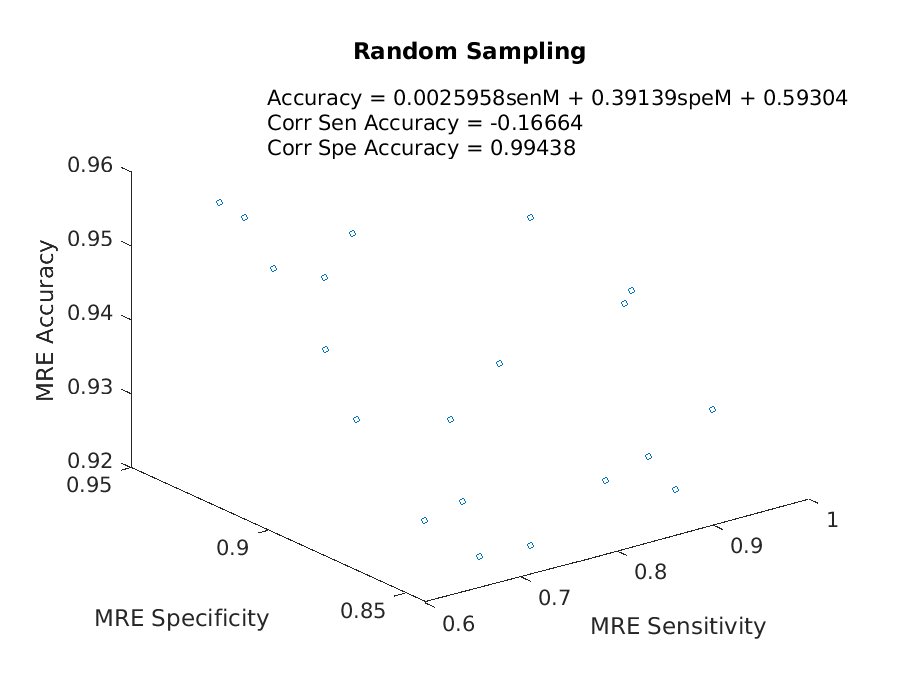
\includegraphics[scale = .3]{mre4}
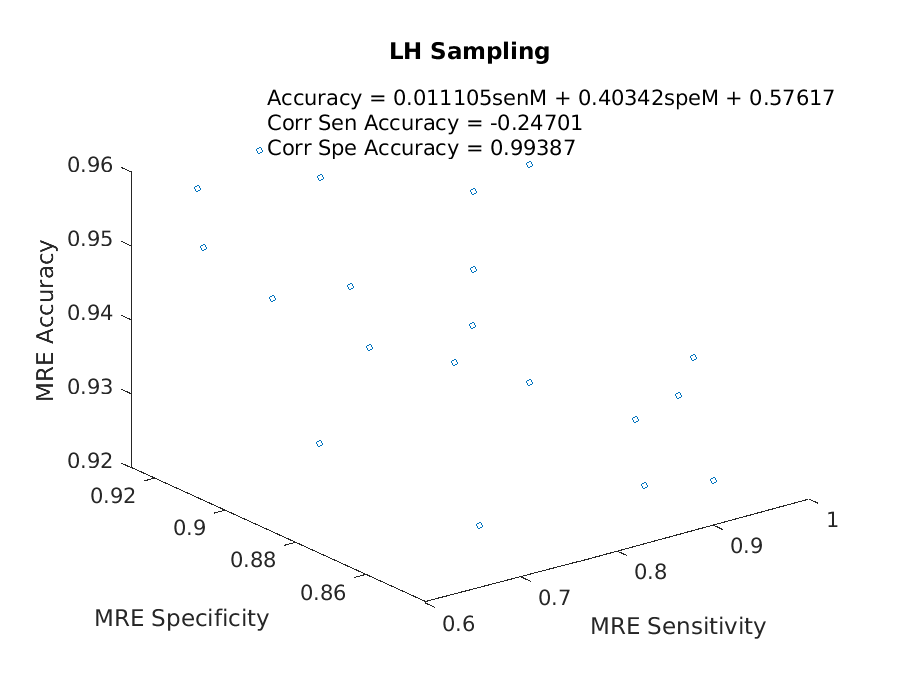
\includegraphics[scale = .3]{mre5}
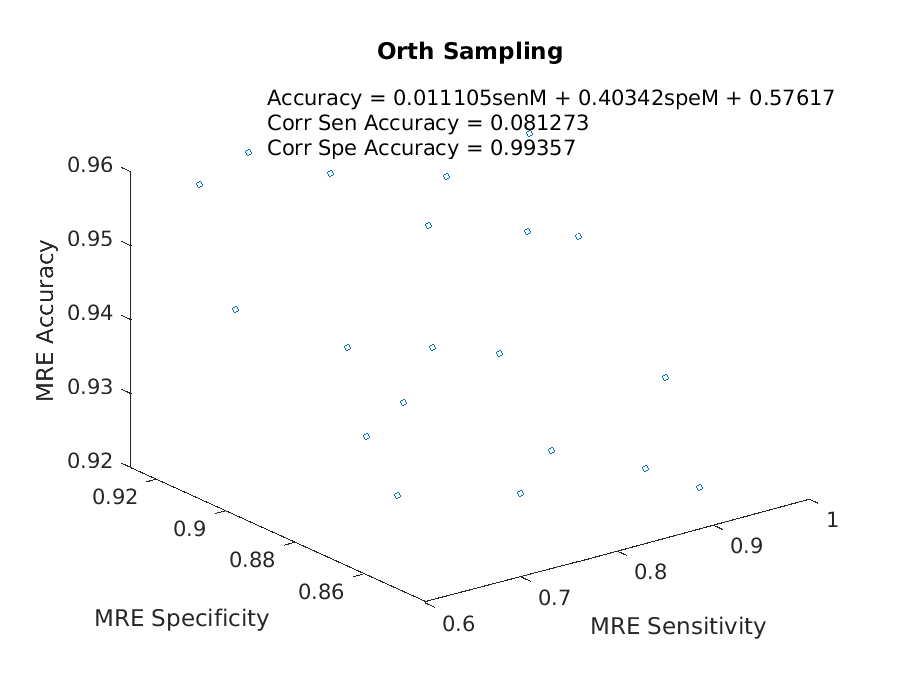
\includegraphics[scale = .3]{mre6}
\end{frame}

\begin{frame}
\frametitle{Question 3f $|$ Sample-Based Sensitivity Analysis for \underline{LB}}
Here are the 3D plots, regression equations and Pearson's correlation coefficients for the LB sample-based Sensitivity Analysis. 

\vspace{1em}
\centering                                                         
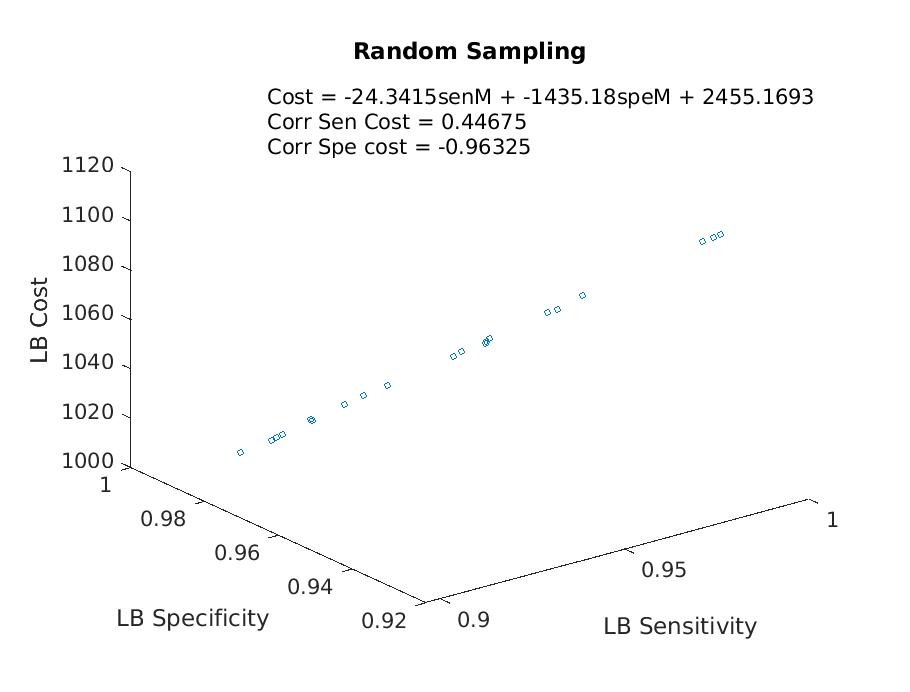
\includegraphics[scale = .3]{lb1}
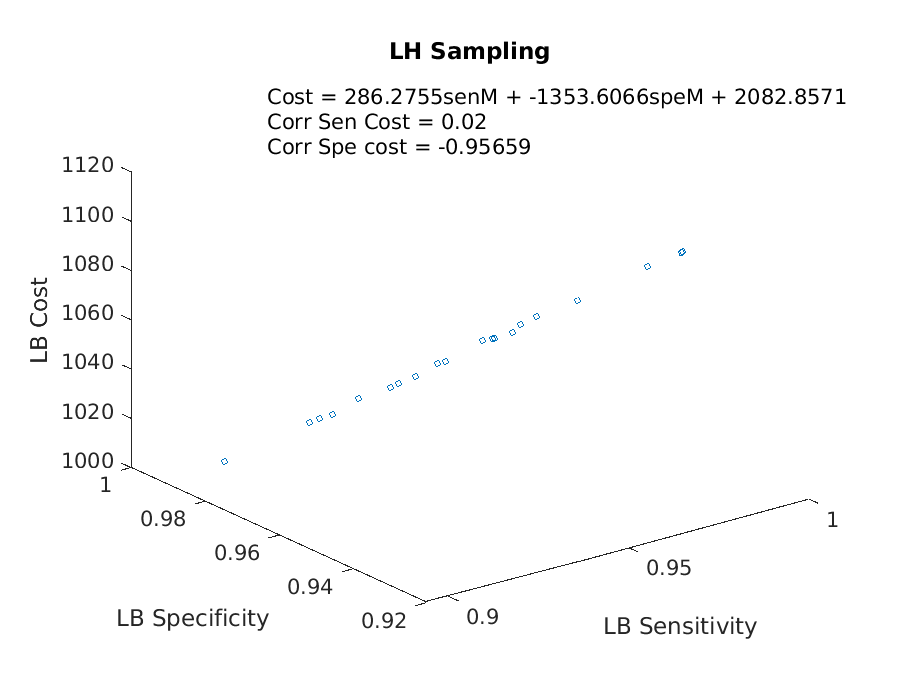
\includegraphics[scale = .3]{lb2}
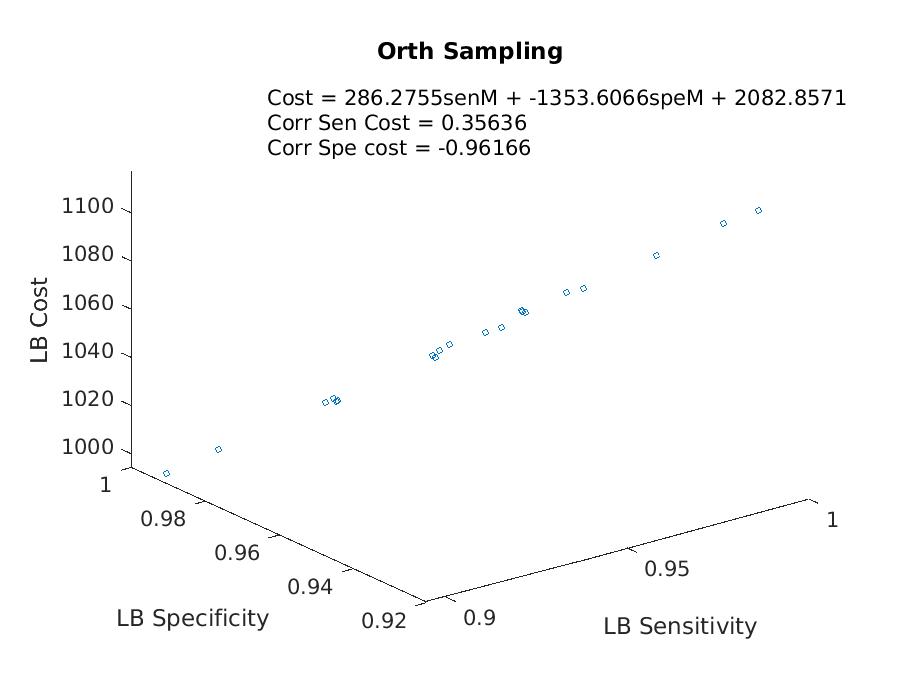
\includegraphics[scale = .3]{lb3}\\
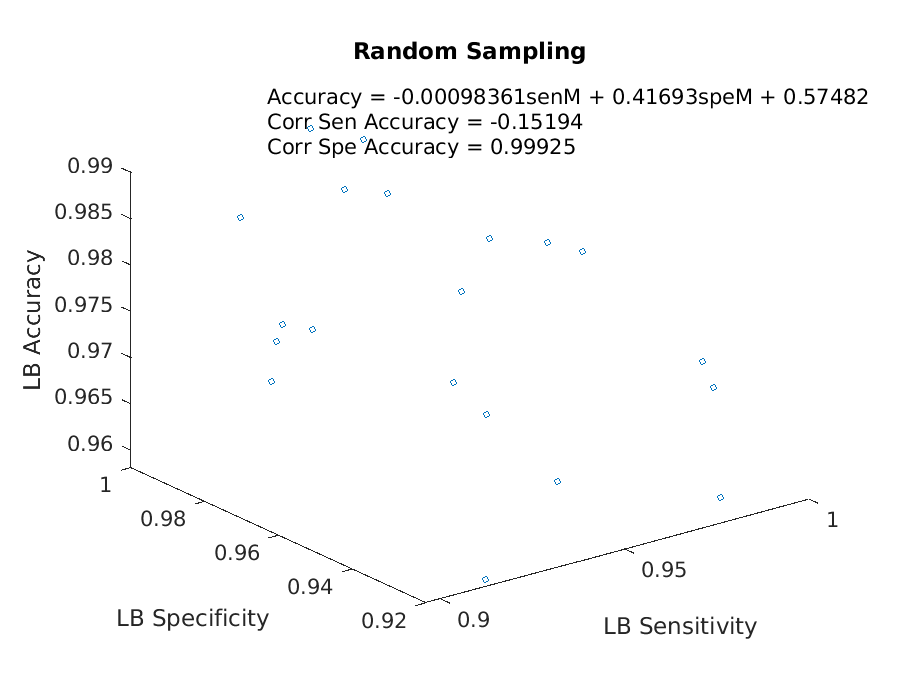
\includegraphics[scale = .3]{lb4}
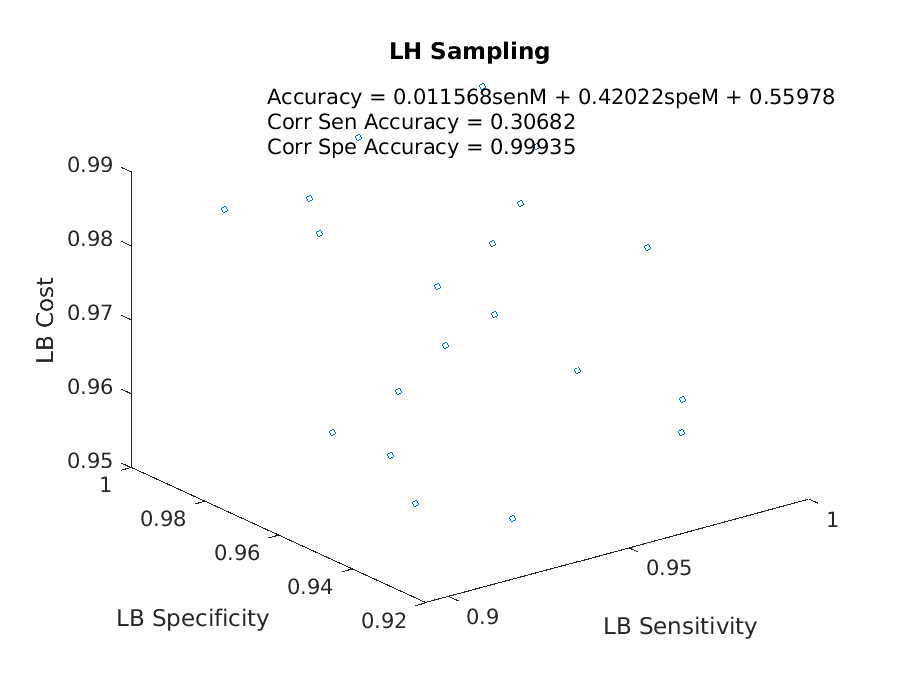
\includegraphics[scale = .3]{lb5}
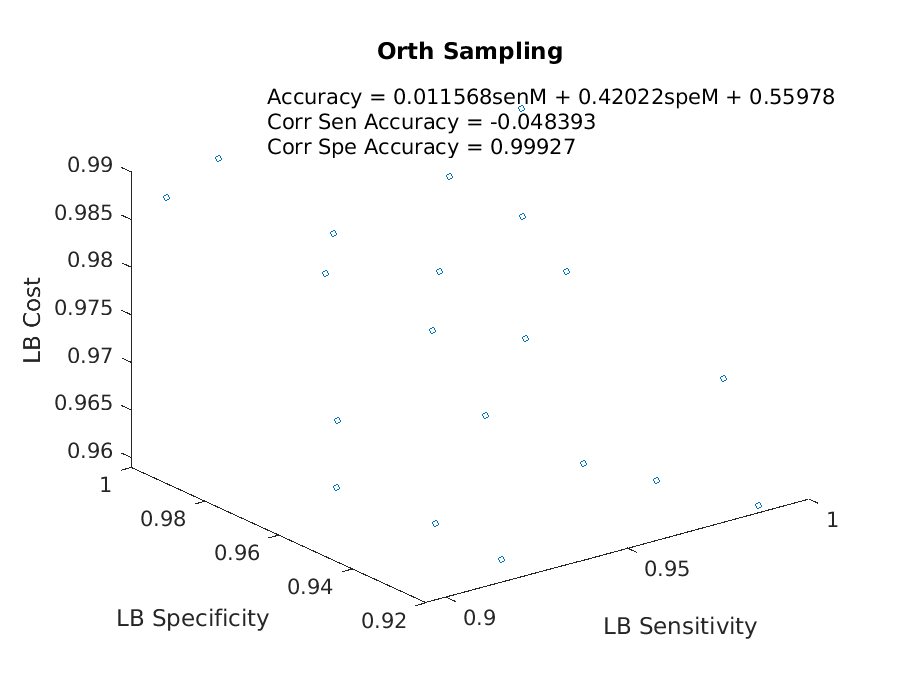
\includegraphics[scale = .3]{lb6}
\end{frame}

\begin{frame}
\frametitle{Question 3g $|$ Rank/Statistical Tests}

Rank transformations may be useful for particular sensitivity analyses, but depend on the type of data and sample selection. In grid-based techniques, the model outputs may have a sort of distribution or cluster of interest. With a rank transformation, visualizing this will be difficult, since the data is transformed to a uniform distribution.

\vspace{1em}
Similarly, statistical tests may be employed when proper assumptions hold true. In this model, the outputs may not be normally distributed (as in the Fib + MRE/LB Accuracy full-factorial experiment). 
\end{frame}

\begin{frame}[shrink = 12]
\frametitle{Question 3h $|$ Inducing Correlation in Sampling}
\setbeamercolor{block title}{use=structure,fg=white,bg=purple!75!black}

Here is a verification that my sampling correlation was induced properly:

\vspace{1em}
\centering                                                         
\includegraphics[width = .32\textwidth]{corr_ex1}
\includegraphics[width = .32\textwidth]{corr_ex2}
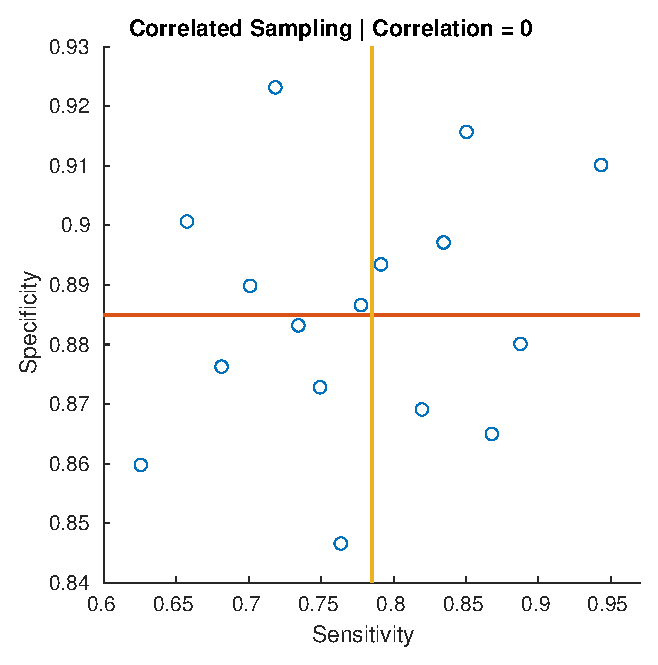
\includegraphics[width = .32\textwidth]{corr_ex3}\\

\begin{columns}
\begin{column}{0.5\textwidth}
\footnotesize{I chose these sampling correlations since there should in theory be a fairly strong correlation between sensitivity and specificity for a good clinical test. However, in some cases, they may not have as much correlation or be weakly correlated. I also assumed a normal distribution of sampling, since these test results are likely also normally distributed.} 
\end{column}
\begin{column}{0.5\textwidth}
\begin{block}{Correction!}
In reality there is more often a trade-off between sensitivity and specificity (not all clinical tests are perfect). Would have been more realistic to have shifted sampling to more properly represent ROC curve! 
\end{block}
\end{column}
\end{columns}
\end{frame}





\begin{frame}
\frametitle{Question 3h $|$ Inducing Correlation in Sampling - \underline{MRE}}

Here are the results with correlated sampling for MRE sens/spec. Correlation decreases from left to right.

\vspace{1em}
\centering                                                         
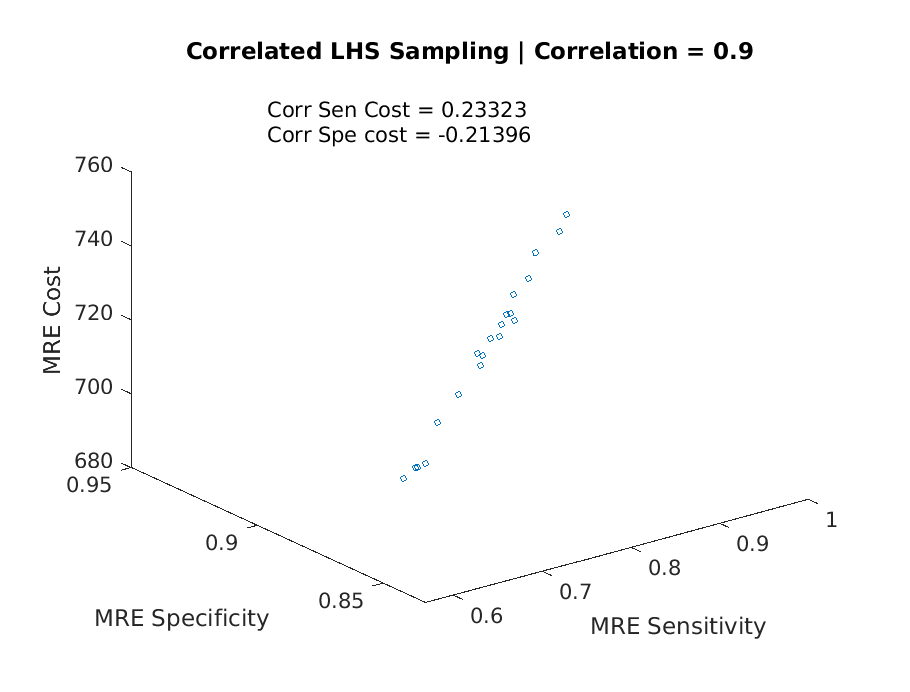
\includegraphics[scale = .3]{mrecorr1}
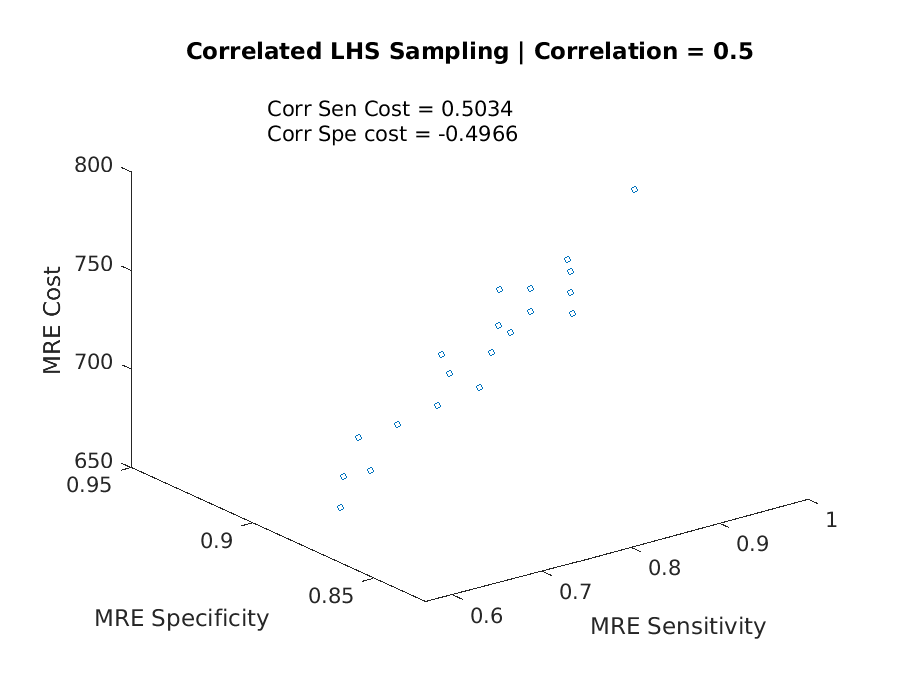
\includegraphics[scale = .3]{mrecorr2}
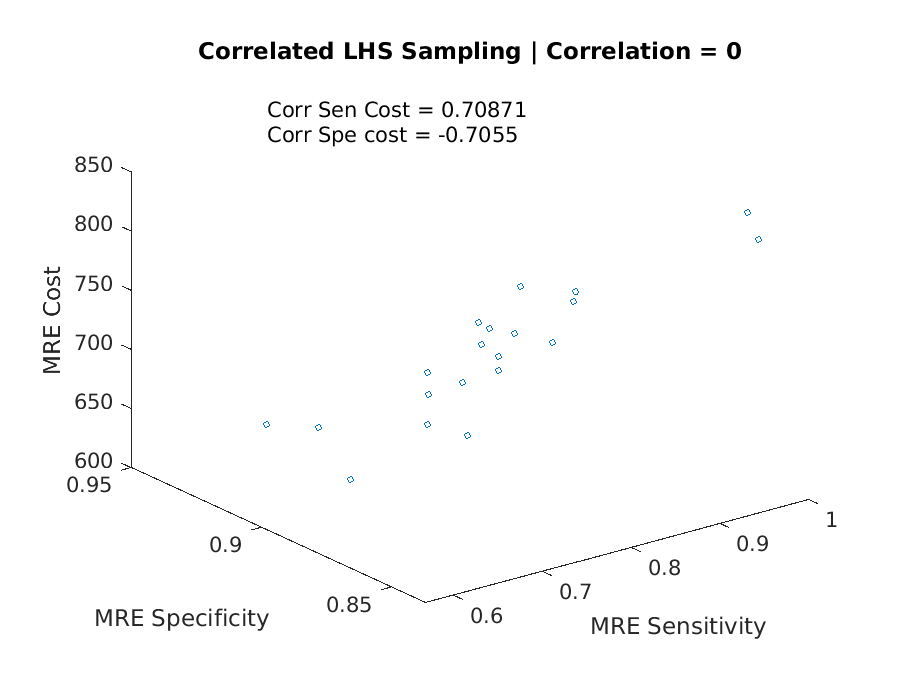
\includegraphics[scale = .3]{mrecorr3}\\
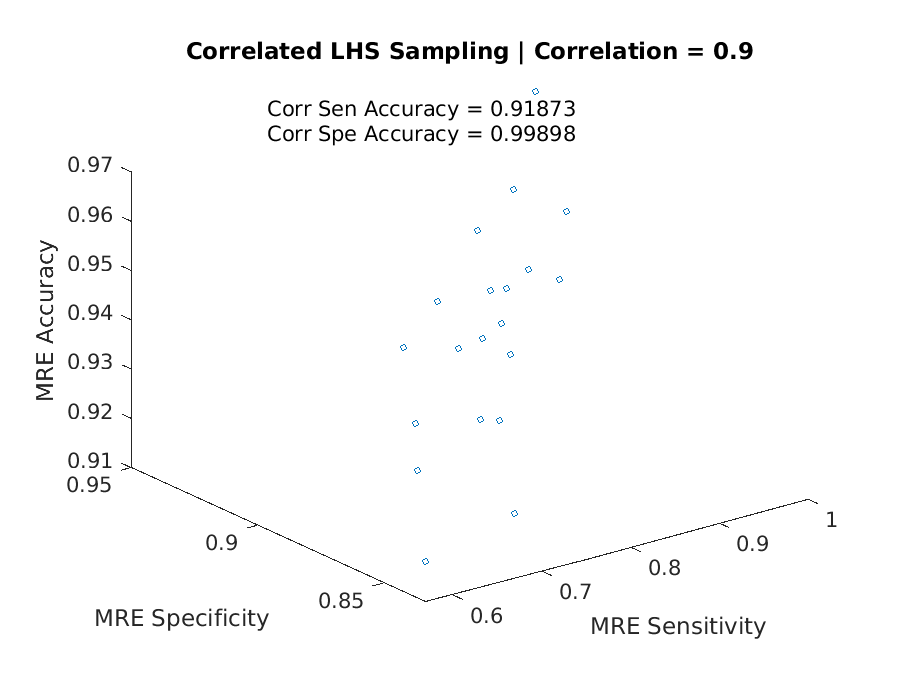
\includegraphics[scale = .3]{mrecorr4}
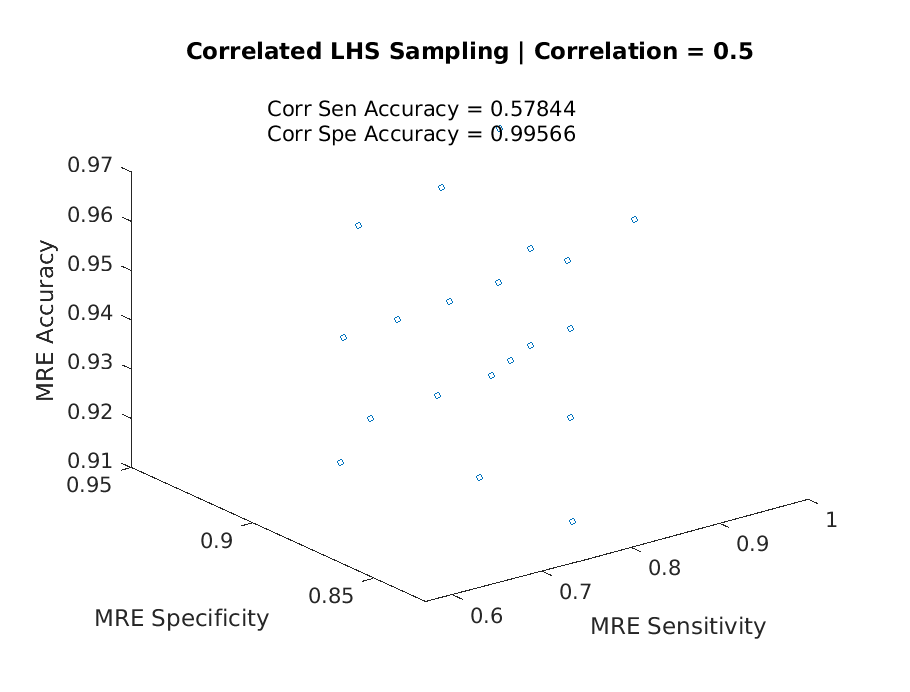
\includegraphics[scale = .3]{mrecorr5}
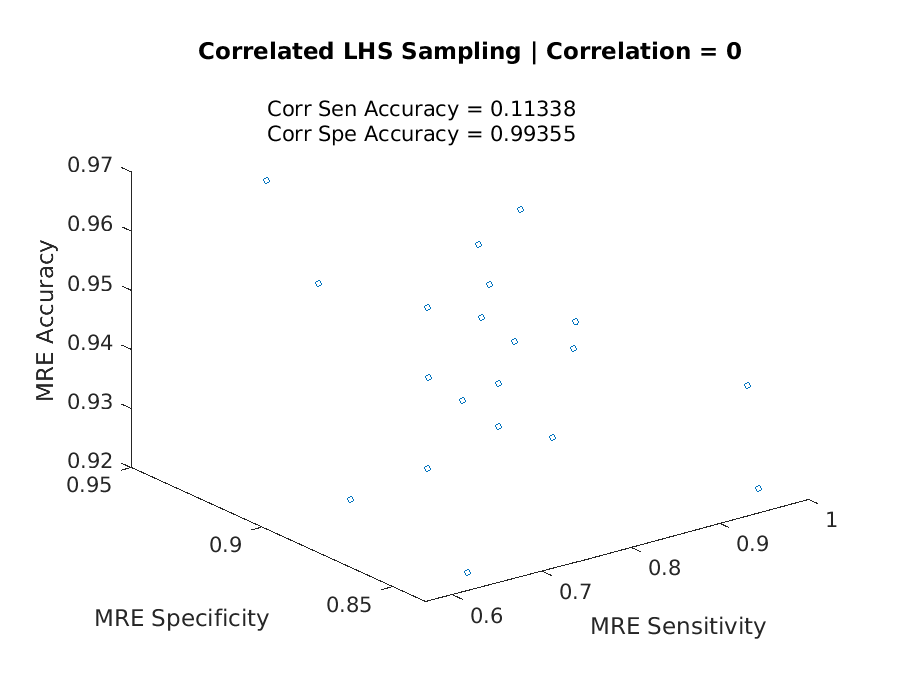
\includegraphics[scale = .3]{mrecorr6}
\end{frame}


\begin{frame}
\frametitle{Question 3h $|$ Inducing Correlation in Sampling - \underline{LB}}

Here are the results with correlated sampling for LB sens/spec. Correlation decreases from left to right.

\vspace{1em}
\centering                                                         
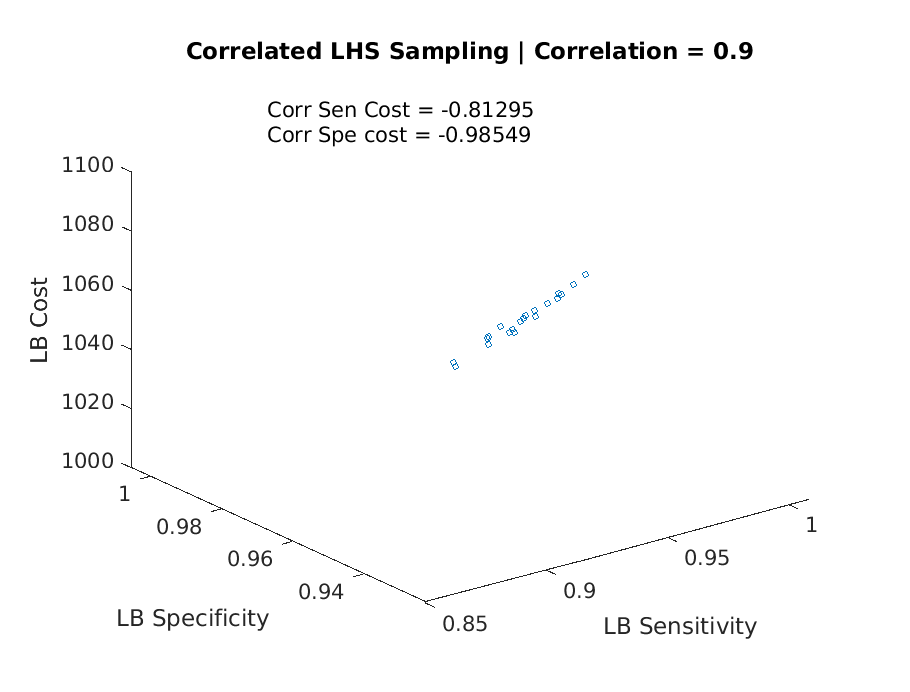
\includegraphics[scale = .3]{lbcorr1}
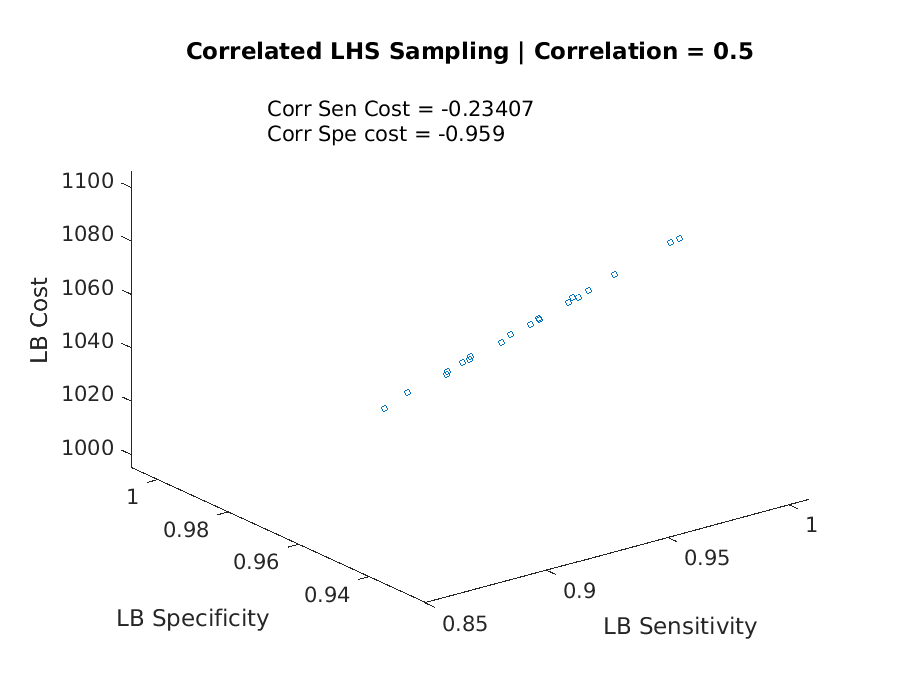
\includegraphics[scale = .3]{lbcorr2}
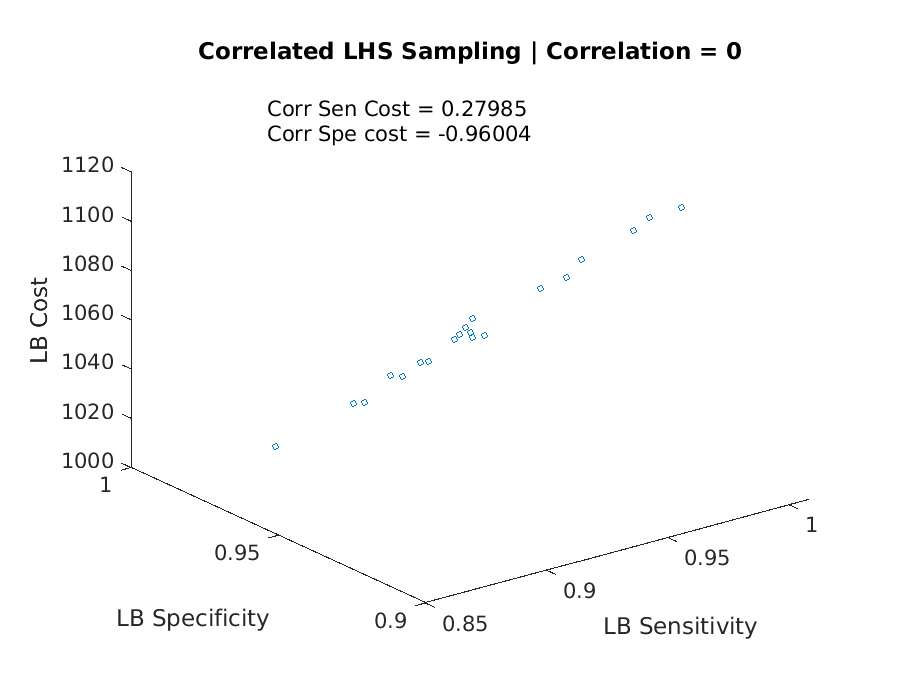
\includegraphics[scale = .3]{lbcorr3}\\
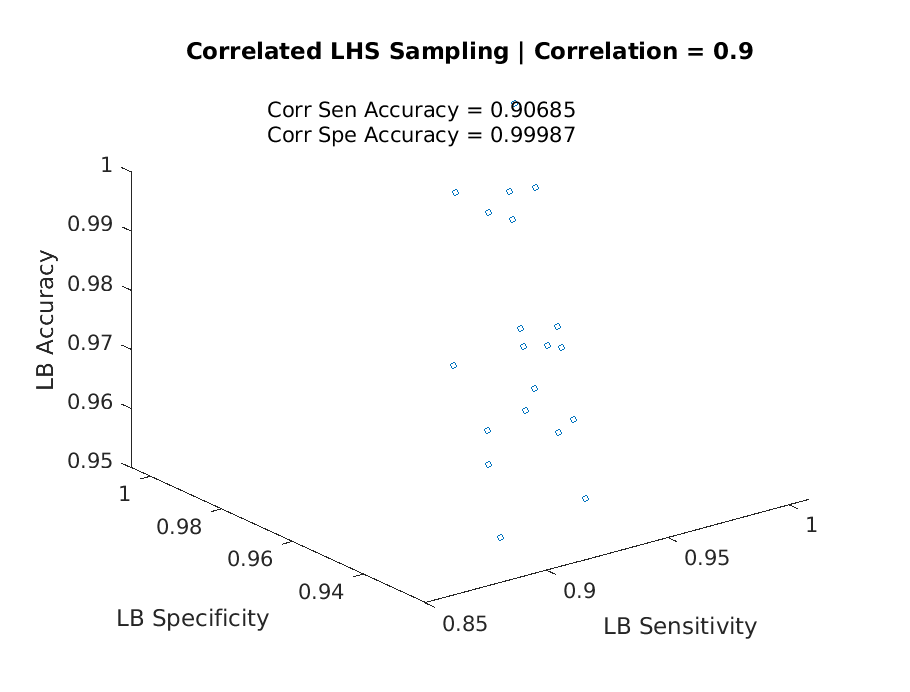
\includegraphics[scale = .3]{lbcorr4}
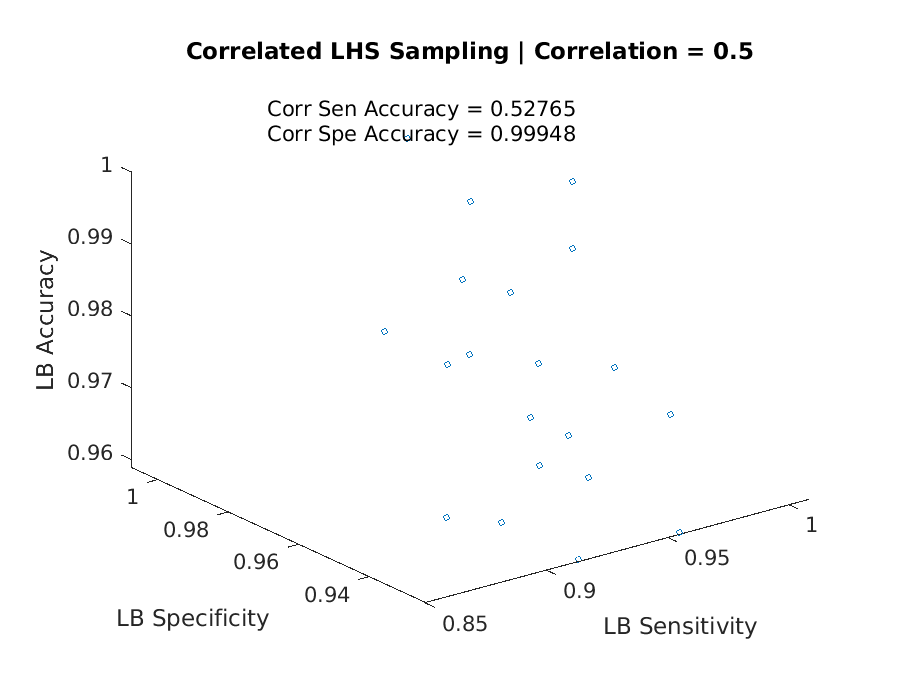
\includegraphics[scale = .3]{lbcorr5}
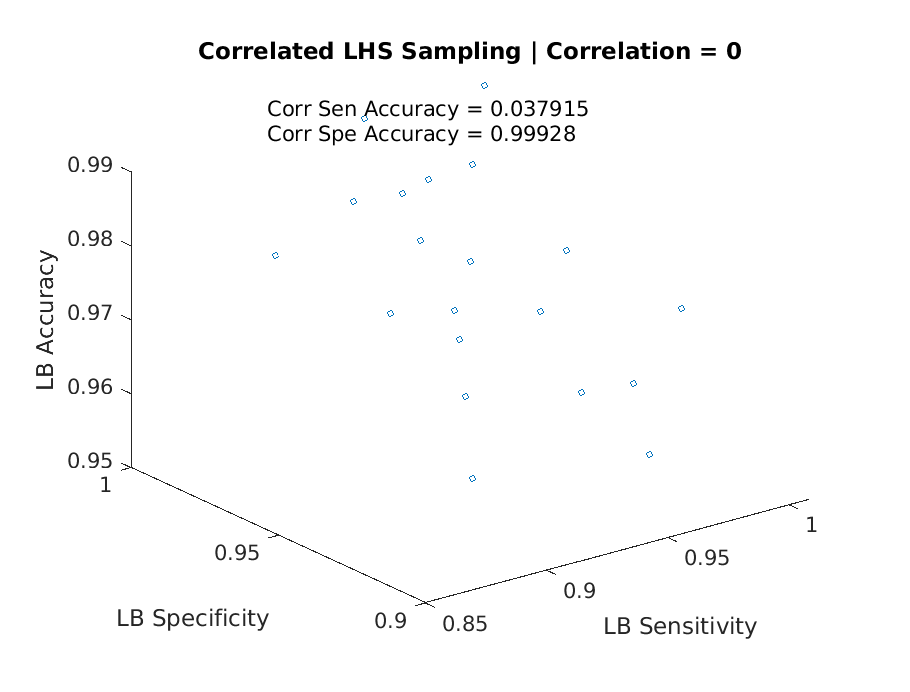
\includegraphics[scale = .3]{lbcorr6}

\end{frame}


\begin{frame}
\frametitle{Question 3i $|$ Importance Sampling}

I changed my sampling distribution from uniform (as in random, lhs, orthogonal sampling). I used a Beta($\alpha,\beta$) distribution with $\alpha = 5$ and $\beta = 2$ for both MRE specificity and senstivity to simulate a more optimistic sampling distribution. This beta distribution implies that the model output means are representative of samples with left-skewed sensitivity and specificity.

\begin{columns}
\begin{column}{0.45\textwidth}
The distributions compared to the uniform distribution found in the LHS sampling technique
\end{column}
\begin{column}{0.45\textwidth}
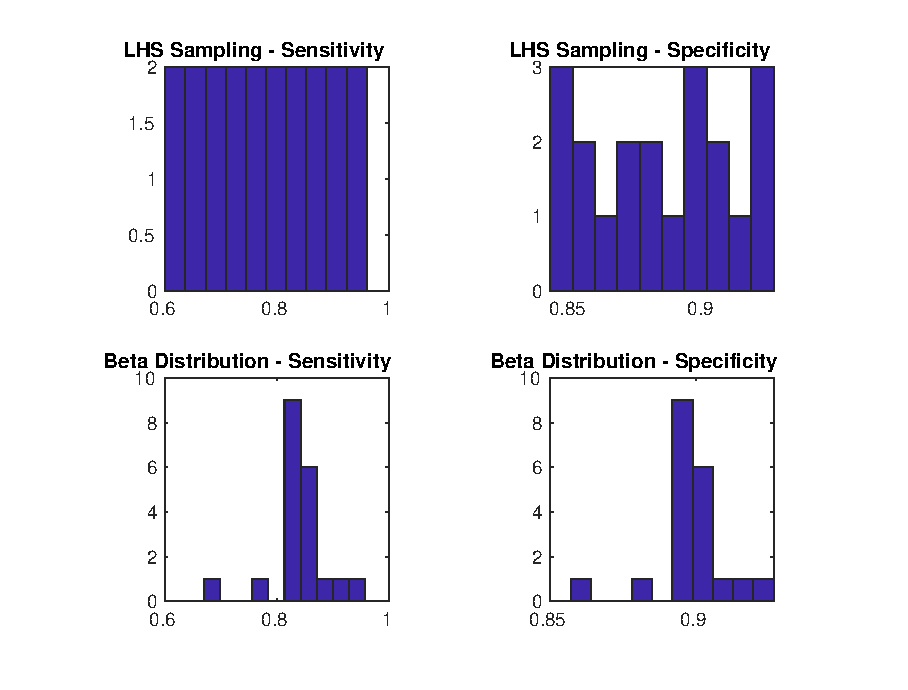
\includegraphics[scale = 0.5]{beta_dist} 
\end{column}
\end{columns}
\end{frame}

\begin{frame}
\frametitle{Question 3i $|$ Importance Sampling}
The output averages were as follows:
\vspace{1em}
\begin{table}[htbp]
\begin{tabular}{|l|l|l|}
\hline
 & \multicolumn{ 2}{l|}{\textbf{\hspace{1em} Parameter Varied}} \\ \hline
 & \textbf{MRE Sens} & \textbf{MRE Spec} \\ \hline
\textbf{Cost} & \multicolumn{1}{r|}{767.0697} & \multicolumn{1}{r|}{706.8664} \\ \hline
\textbf{Accuracy} & \multicolumn{1}{r|}{0.9324} & \multicolumn{1}{r|}{0.9471} \\ \hline
\end{tabular}\end{table}
\vspace{1em}
As sensitivity is skewed left, the accuracy decreases and cost increases. Conversely, as specificity is skewed left, the accuracy increases, and the cost decreases. This could be because a higher positive test rate (true in screening tests with higher sensitivity) results in a required confirmatory test with another method with additional costs. A more specific test means less false positives, which prevents decreases the likelihood of this added cost.  
\end{frame}
\end{document}